\documentclass{article}
\author{Lin Jiaying}
\title{Assignment 3 of The design and Analysis of Computer Algorithms}
\usepackage{tikz}
\usepackage{tabu}
\usepackage{caption}
\usepackage{algorithm}
\usepackage{cite}
\usepackage{algorithmic}
\usepackage{amsmath}
\usetikzlibrary{positioning}
\renewcommand{\algorithmicrequire}{\textbf{Input:}} 
\renewcommand{\algorithmicensure}{\textbf{Output:}}
\tikzset{main node/.style={circle,draw,minimum size=1cm,inner sep=0pt},
}

\begin{document}
	\maketitle
	%\clearpage
	\section{Question3.1}
	\paragraph{3.1}
		Using Kruskal's algorithm to find a minimum spanning tree of the following graph.\\
	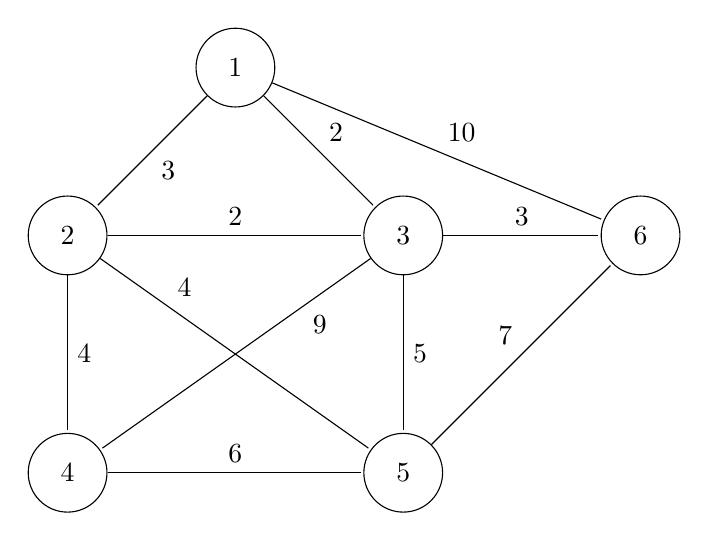
\begin{tikzpicture}[node distance = 2.0cm,auto, shorten >= 1pt]
		\node[main node] (1){$1$};
		\node[main node] (2)[below left = of 1]{$2$};
		\node[main node] (3)[below right = of 1]{$3$};
		\node[main node] (6)[right = of 3]{$6$};
		\node[main node] (4)[below = of 2]{$4$};
		\node[main node] (5)[below = of 3]{$5$};
		
		
		\path[draw]
		(1) edge node {3} (2)
		(1) edge node {2} (3)
		(1) edge node {10} (6)
		(2) edge node {2} (3)
		(3) edge node {3} (6)
		(2) edge node {4} (4)
		(4) edge node {6} (5)
		(5) edge node {7}  (6)
		(3) edge node[near start] {9} (4)
		(2) edge node[near start] {4} (5)
		(3) edge node {5} (5);
	\end{tikzpicture}
	\paragraph{3.1 Answer:}
	\paragraph{Step 1:}
		First, we need to sort all edges in this graph, easily we get a sequence in this pattern like Example 3-2 in textbook. \\
		(1,3) -- weight 2\\
		(2,3) -- weight 2\\
		(1,2) -- weight 3\\
		(3,6) -- weight 3\\
		(2,5) -- weight 4\\
		(2,4) -- weight 4\\
		(3,5) -- weight 5\\
		(4,5) -- weight 6\\
		(5,6) -- weight 7\\
		(3,4) -- weight 9\\
		(1,6) -- weight 10\\
		
	\paragraph{Step 2:}	
		We add (1,3) edge  into the tree since it has a smallest weight in current E and then check if there is a cycle in the spanning tree. After adding the edge(1,3), we delete it from set E.\\
	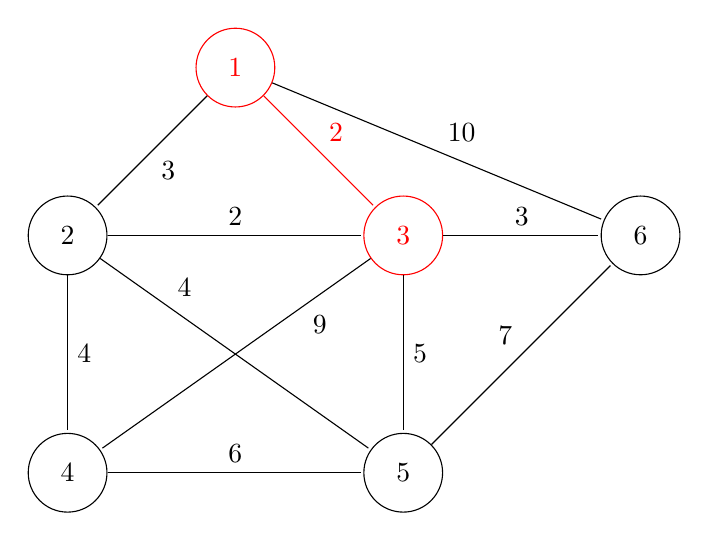
\begin{tikzpicture}[node distance = 2.0cm,auto, shorten >= 1pt]
	\node[main node,red] (1){$1$};
	\node[main node] (2)[below left = of 1]{$2$};
	\node[main node,red] (3)[below right = of 1]{$3$};
	\node[main node] (6)[right = of 3]{$6$};
	\node[main node] (4)[below = of 2]{$4$};
	\node[main node] (5)[below = of 3]{$5$};
	
	
	\path[draw]
	(1) edge node {3} (2)
	(1) edge[red] node {2} (3)
	(1) edge node {10} (6)
	(2) edge node {2} (3)
	(3) edge node {3} (6)
	(2) edge node {4} (4)
	(4) edge node {6} (5)
	(5) edge node {7}  (6)
	(3) edge node[near start] {9} (4)
	(2) edge node[near start] {4} (5)
	(3) edge node {5} (5);
	\end{tikzpicture}
	
	\paragraph{Step 3:}
			We add (2,3) edge  into the tree since it has a smallest weight in current E and then check if there is a cycle in the spanning tree. After adding the edge(2,3), we delete it from set E.\\	
		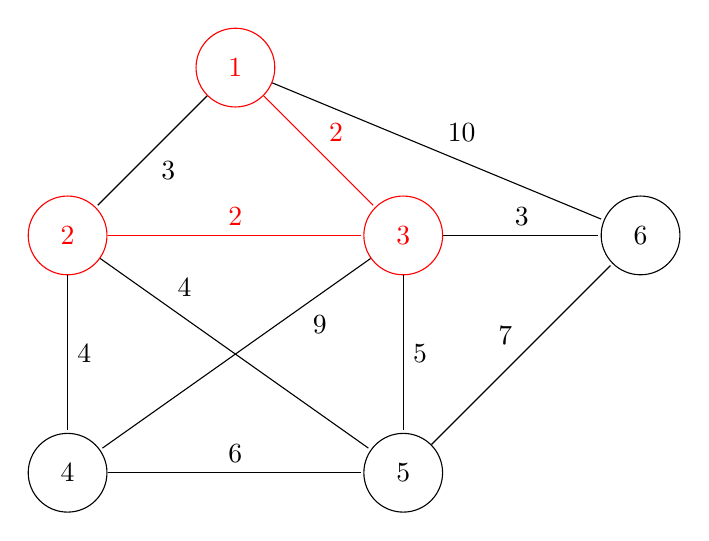
\begin{tikzpicture}[node distance = 2.0cm,auto, shorten >= 1pt]
	\node[main node,red] (1){$1$};
	\node[main node,red] (2)[below left = of 1]{$2$};
	\node[main node,red] (3)[below right = of 1]{$3$};
	\node[main node] (6)[right = of 3]{$6$};
	\node[main node] (4)[below = of 2]{$4$};
	\node[main node] (5)[below = of 3]{$5$};
	
	
	\path[draw]
	(1) edge node {3} (2)
	(1) edge[red] node {2} (3)
	(1) edge node {10} (6)
	(2) edge[red] node {2} (3)
	(3) edge node {3} (6)
	(2) edge node {4} (4)
	(4) edge node {6} (5)
	(5) edge node {7}  (6)
	(3) edge node[near start] {9} (4)
	(2) edge node[near start] {4} (5)
	(3) edge node {5} (5);
	\end{tikzpicture}
		\paragraph{Step 4:}
	We add (1,2) edge  into the tree since it has a smallest weight in current E and then check if there is a cycle in the spanning tree, but we find that it may cause a cycle to add this edge, so we discard it.\\	
	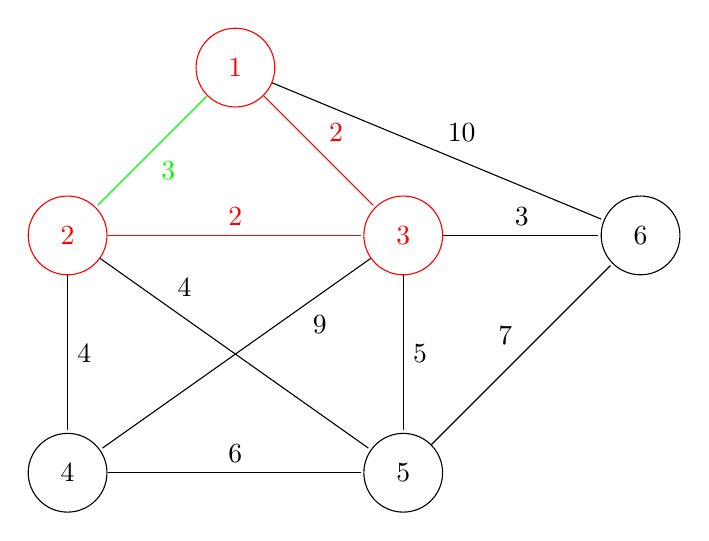
\begin{tikzpicture}[node distance = 2.0cm,auto, shorten >= 1pt]
	\node[main node,red] (1){$1$};
	\node[main node,red] (2)[below left = of 1]{$2$};
	\node[main node,red] (3)[below right = of 1]{$3$};
	\node[main node] (6)[right = of 3]{$6$};
	\node[main node] (4)[below = of 2]{$4$};
	\node[main node] (5)[below = of 3]{$5$};
	
	
	\path[draw]
	(1) edge[green] node {3} (2)
	(1) edge[red] node {2} (3)
	(1) edge node {10} (6)
	(2) edge[red] node {2} (3)
	(3) edge node {3} (6)
	(2) edge node {4} (4)
	(4) edge node {6} (5)
	(5) edge node {7}  (6)
	(3) edge node[near start] {9} (4)
	(2) edge node[near start] {4} (5)
	(3) edge node {5} (5);
	\end{tikzpicture}	
			\paragraph{Step 5:}
	We add (3,6) edge  into the tree since it has a smallest weight in current E and then check if there is a cycle in the spanning tree, after checking there's no cycle, we add it to the tree and delete it from the set E.\\	
	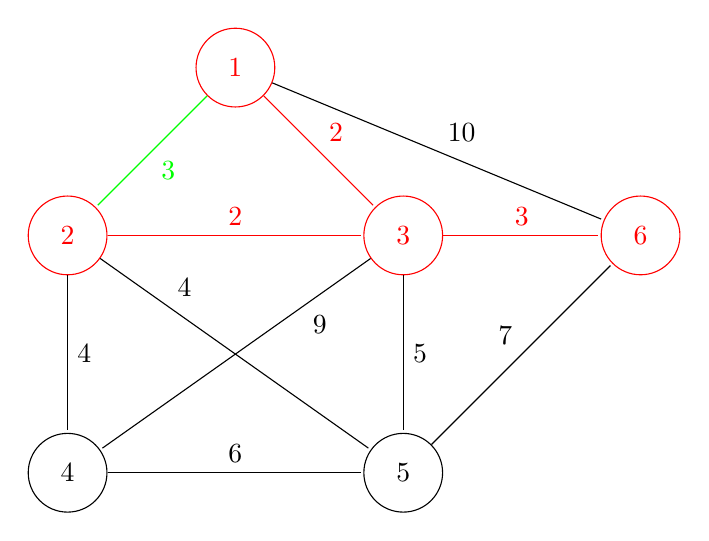
\begin{tikzpicture}[node distance = 2.0cm,auto, shorten >= 1pt]
	\node[main node,red] (1){$1$};
	\node[main node,red] (2)[below left = of 1]{$2$};
	\node[main node,red] (3)[below right = of 1]{$3$};
	\node[main node,red] (6)[right = of 3]{$6$};
	\node[main node] (4)[below = of 2]{$4$};
	\node[main node] (5)[below = of 3]{$5$};
	
	
	\path[draw]
	(1) edge[green] node {3} (2)
	(1) edge[red] node {2} (3)
	(1) edge node {10} (6)
	(2) edge[red] node {2} (3)
	(3) edge[red] node {3} (6)
	(2) edge node {4} (4)
	(4) edge node {6} (5)
	(5) edge node {7}  (6)
	(3) edge node[near start] {9} (4)
	(2) edge node[near start] {4} (5)
	(3) edge node {5} (5);
	\end{tikzpicture}	
		\paragraph{Step 6:}
	We add (2,4) edge  into the tree since it has a smallest weight in current E and then check if there is a cycle in the forest, after checking there's no cycle, we add it to the tree and delete it from the set E.\\	
	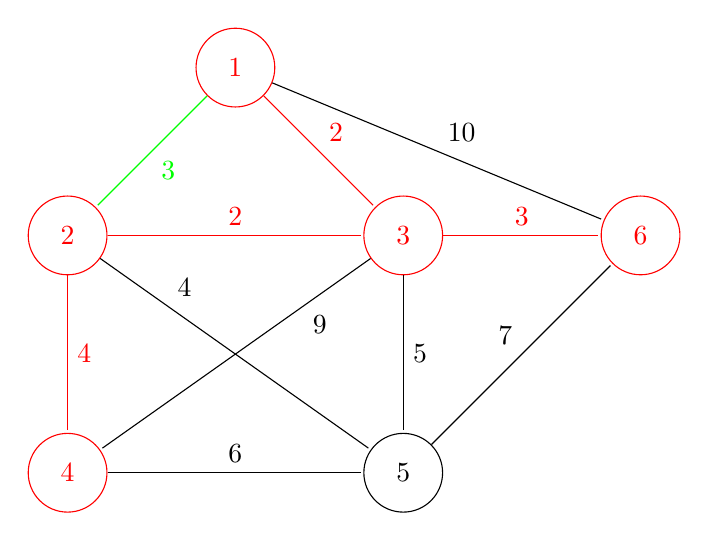
\begin{tikzpicture}[node distance = 2.0cm,auto, shorten >= 1pt]
	\node[main node,red] (1){$1$};
	\node[main node,red] (2)[below left = of 1]{$2$};
	\node[main node,red] (3)[below right = of 1]{$3$};
	\node[main node,red] (6)[right = of 3]{$6$};
	\node[main node,red] (4)[below = of 2]{$4$};
	\node[main node] (5)[below = of 3]{$5$};
	
	
	\path[draw]
	(1) edge[green] node {3} (2)
	(1) edge[red] node {2} (3)
	(1) edge node {10} (6)
	(2) edge[red] node {2} (3)
	(3) edge[red] node {3} (6)
	(2) edge[red] node {4} (4)
	(4) edge node {6} (5)
	(5) edge node {7}  (6)
	(3) edge node[near start] {9} (4)
	(2) edge node[near start] {4} (5)
	(3) edge node {5} (5);
	\end{tikzpicture}	
			\paragraph{Step 7:}
	We add (2,5) edge  into the tree since it has a smallest weight in current E and then check if there is a cycle in the spanning tree, after checking there's no cycle, we add it to the tree and delete it from the set E.\\	
	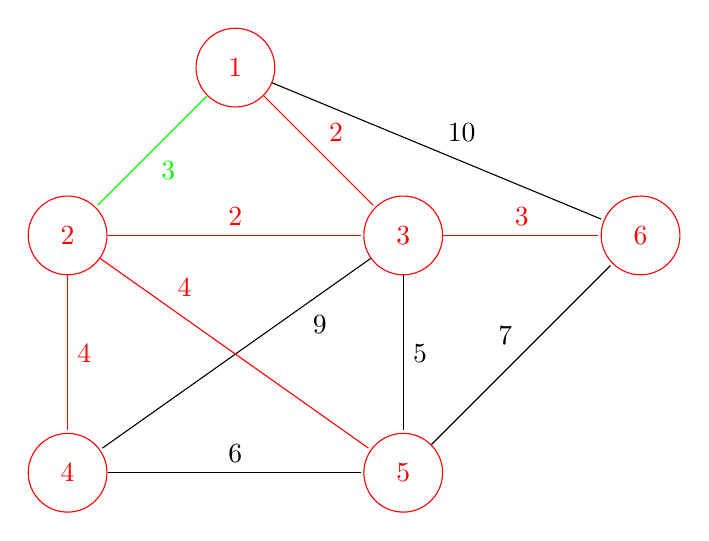
\begin{tikzpicture}[node distance = 2.0cm,auto, shorten >= 1pt]
	\node[main node,red] (1){$1$};
	\node[main node,red] (2)[below left = of 1]{$2$};
	\node[main node,red] (3)[below right = of 1]{$3$};
	\node[main node,red] (6)[right = of 3]{$6$};
	\node[main node,red] (4)[below = of 2]{$4$};
	\node[main node,red] (5)[below = of 3]{$5$};
	
	
	\path[draw]
	(1) edge[green] node {3} (2)
	(1) edge[red] node {2} (3)
	(1) edge node {10} (6)
	(2) edge[red] node {2} (3)
	(3) edge[red] node {3} (6)
	(2) edge[red] node {4} (4)
	(4) edge node {6} (5)
	(5) edge node {7}  (6)
	(3) edge node[near start] {9} (4)
	(2) edge[red] node[near start] {4} (5)
	(3) edge node {5} (5);
	\end{tikzpicture}
	\paragraph{Step 8:}
	Finally we find that now the spanning tree has N - 1(5) edges and we stop generating the tree. The minimum spanning tree is showed as followed.\\
	\begin{tikzpicture}[node distance = 2.0cm,auto, shorten >= 1pt]
	\node[main node,red] (1){$1$};
	\node[main node,red] (2)[below left = of 1]{$2$};
	\node[main node,red] (3)[below right = of 1]{$3$};
	\node[main node,red] (6)[right = of 3]{$6$};
	\node[main node,red] (4)[below = of 2]{$4$};
	\node[main node,red] (5)[below = of 3]{$5$};
	
	
	\path[draw]
	%(1) edge[green] node {3} (2)
	(1) edge[red] node {2} (3)
%	(1) edge node {10} (6)
	(2) edge[red] node {2} (3)
	(3) edge[red] node {3} (6)
	(2) edge[red] node {4} (4)
	%(4) edge node {6} (5)
	%(5) edge node {7}  (6)
	%(3) edge node[near start] {9} (4)
	(2) edge[red] node[near start] {4} (5);
	%(3) edge node {5} (5);
	\end{tikzpicture}
	
	\section{Question 3.7}
	\paragraph{3.7:}
	Using Dijkstra's algorithm to find the shortest paths from $V_1$ to all notes.\\
	\paragraph{3.7 Answer:}
	The graph is shown as follows.\\
	\\
	\\
	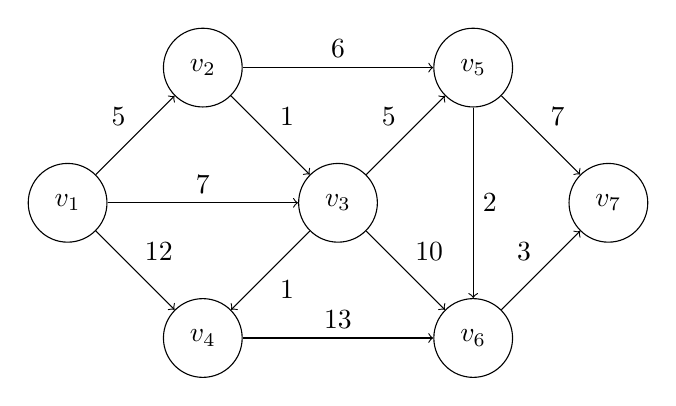
\begin{tikzpicture}[auto]
		\node[main node] (v1) {$v_1$};
		\node[main node](v2) [above right = of v1]{$v_2$};
		\node[main node](v4) [below right = of v1]{$v_4$};
		\node[main node](v3) [below right = of v2]{$v_3$};
		\node[main node](v5) [above right = of v3]{$v_5$};
		\node[main node](v6) [below right = of v3]{$v_6$};
		\node[main node](v7) [below right = of v5]{$v_7$};
		
		\path[->]
			(v1) edge node {5} (v2)
			(v1) edge node {12} (v4)
			(v1) edge node {7} (v3)
			(v2) edge node {1} (v3)
			(v2) edge node {6} (v5)
			(v3) edge node {5} (v5)
			(v3) edge node {1} (v4)
			(v3) edge node {10} (v6)
			(v5) edge node {2} (v6)
			(v5) edge node {7} (v7)
			(v4) edge node {13} (v6)
			(v6) edge node {3} (v7);
	\end{tikzpicture}
	\\
	The Dijkstra's algorithm will process as follows:\\
	
	\paragraph{Step 1:}.\\
	\\
	$S = \{v_1\}$\\
	$L(v_2) = 5$\\
	$L(v_3) = 7$\\
	$L(v_4) = 12$\\
	All of the other $L(v_i) $'s are equal to $\infty$.\\
	$L(v_2) $ is the smallest. $v_1v_2$ is the shortest path from $v_1$ to $v_2$.\\
	$S = \{v_1, v_2\}$\\
	
	\paragraph{Step 2:}. \\
	\\
\begin{align*}  
	L(v_3) &= min(7, L(v_2) + c(v_2, v_3) \\  
	&= min(7, 5 + 1)  \\  
	&= 6\\
	L(v_5) &= min(\infty, L(v_2) + c(v_2, v_5) \\  
	&= 5 + 6  \\  
	&= 11\\	
\end{align*}  
	$L(v_3) $ is the smallest. $v_1v_2v_3$ is the shortest path from $v_1$ to $v_3$.\\
$S = \{v_1, v_2, v_3\}$\\

	\paragraph{Step 3:} .\\
	\\
	\begin{align*}
	L(v_4) &= min(12, L(v_3) + c(v_3, v_4)) \\
	&= min(12, 6 + 1)\\
	&= 7\\
	L(v_5) &= min(11, L(v_3) + c(v_3, v_5))\\
	&= min(11, 6 + 5)\\
	&= 11\\
	L(v_6) &= min(\infty, L(v_3) + c(v_3, v_6))\\
	&= 6 + 10\\
	&= 16\\	
		content...
	\end{align*}
		$L(v_4) $ is the smallest. $v_1v_2v_3v_4$ is the shortest path from $v_1$ to $v_4$.\\
	$S = \{v_1, v_2, v_3, v_4\}$\\	
	
	\paragraph{Step 4:} .\\
	\\
	\begin{align*}
		L(v_6) &= min(16, L(v_4) + c(v_4, v_6))\\
	&= min(16, 7 + 13)\\
	&= 16\\
	L(v_5) &= 11\\
	\end{align*}

			
	$L(v_5) $ is the smallest. $v_1v_2v_3v_5$ is the shortest path from $v_1$ to $v_5$.\\
	$S = \{v_1, v_2, v_3, v_4, v_5\}$\\	
	
	\paragraph{Step 5:} .\\
		\\
	\begin{align*}
	L(v_6) &= min(16, L(v_5) + c(v_5, v_6))\\
&= min(16, 11 + 2)\\
&= 13\\
L(v_7) &= min(\infty, L(v_5) + c(v_5, v_7)\\
&= 11 + 7\\
&= 18\\
	\end{align*}

		$L(v_6) $ is the smallest. $v_1v_2v_3v_5v_6$ is the shortest path from $v_1$ to $v_6$.\\
	$S = \{v_1, v_2, v_3, v_4, v_5, v_6\}$\\
	
	\paragraph{Step 6:} .\\
	\\
	\begin{align*}
	L(v_7) &= min(18, L(v_6) + c(v_6, v_7)\\
	&= min(18, 13 + 3)\\
	&= 16\\	
	\end{align*} %align no empty line
	$L(v_7) $ is the smallest. $v_1v_2v_3v_5v_6v_7$ is the shortest path from $v_1$ to $v_7$.\\
	$S = \{v_1, v_2, v_3, v_4, v_5, v_6, v_7\}$\\
		
	\begin{center}{Table 1 Shortest paths from vertex $v_1$}
	\begin{tabu} to \hsize {X|X}	
	\hline
	Vertex & Shortest distance to $v_1$ (length)\\
	\hline
	$v_2$ & $v_1v_2$ (5)\\
	$v_3$ & $v_1v_2v_3$(5 + 1 = 6)\\
	$v_4$ & $v_1v_2v_3v_4$(6 + 1 = 7)\\
	$v_5$ & $v_1v_2v_3v_4v_5$(6 + 5 = 11)\\
	$v_6$ & $v_1v_2v_3v_5v_6$(11 + 2 = 13)\\
	$v_7$ & $v_1v_2v_3v_5v_6v_7$(13 + 3 = 16)\\
	\hline
\end{tabu}
\end{center}

\begin{table} [!hbp]
	\begin{tabular}{clcccccccc}
	%\hline	
	Iteration& S & Vertex Selected & $v_1$ & $v_2$ & $v_3$ &$v_4$ &$v_5$ &$v_6$ &$v_7$\\
	\hline
	Initial & & -- \\
	%\hline
	1 & $v_1$ & $v_2$ & 0 & 5 &7 & 12 & $+\infty$ & $+\infty$ &$+\infty$ \\
	%\hline
	2 & $v_1, v_2$ & $v_3$ & 0 & 5 & 6 & 12 & 11 & $+\infty$ & $+\infty$\\
	%\hline
	3 & $v_1, v_2, v_3$ & $v_4$ & 0 & 5 & 6 & 7 & 11 & 16  & $+\infty$\\
	%\hline
	4 & $v_1, v_2, v_3, v_4$ & $v_5$ & 0 & 5 & 6 & 7 & 11 & 16 & $+\infty$\\
	
	5 & $v_1, v_2, v_3, v_4, v_5 $ & $v_6$ & 0 & 5 & 6 & 7 & 11 & 13 & 18\\
	6 & $v_1, v_2, v_3, v_4, v_5, v_6$ &$v_7$&  0 & 5 & 6 & 7 & 11 & 13 & 16\\

\end{tabular}
	\end{table}
\section{Question 3.11}
\paragraph{3.11}
	The knapsack problem is defined as follows:\\
	Given positive integers $P_1, P_2, ... , P_n, W_1, W_2, ..., W_n and M$.\\
	Find $X_1, X_2, ..., X_n, 0 \leq X_i \leq 1 $ such that\\
	$\sum_{i=1}^{n} P_iX_i $\\
	is maximized subject to\\
	$\sum_{i=1}^{n}W_iX_i \leq M$.\\
	Give a greedy method to find an optimal solution of the knapsack problem and prove its correctness.
	\paragraph{3.11 Answer:}
	My greedy method is:
	For our solution $X_1, X_2, ..., X_n, 0 \leq X_i \leq 1 $, I denote that the solution is like $S(X_1, X_2, ..., X_i, X_j, ..., X_n) $ which are sorted in descending order by their radio of $\frac{P_i}{W_i}$, so we have $\frac{P_1}{W_1} \geq \frac{P_2}{W_2} \geq ... \geq \frac{P_n}{W_n}$\\
	In our greedy method solution, if $\sum_{i=1}^{n} W_i \leq M$, we make all $X$ equal to 1, obviously it's a optimal solution in this situation.\\
	if$\sum_{i=1}^{n} W_i \geq M$, it means we can't put all items into the packages, at least one package $0 \leq X_j  \leq 1, 0 \leq j \leq n$, since we have sorted the "price/weight" radio and we use greedy method it means that only one package can have a fractional or "one" value, when we detect this value, we can terminate the algorithm, so we can simply summarize that:\\
	\begin{align*}
	X_i &= 1, 0 \leq i < j\\
	X_i &\in (0,1), i = j\\
	X_i &= 0, j < i \leq n\\
	\end{align*}
	The pseudocode of this greedy method is demonstrated as follows:
	\begin{algorithm}
		\caption{A greedy method for this knapsack problem}
		\begin{algorithmic}[1]
		 	\REQUIRE 
		 	$W[1:n]$: n positive integers.\\
		 			 $P[1:n]$:n positive integers.\\
		 			 $M$: an positive integer.\\
		 			 %$X[1:n] $:n real number $\in[0,1] $.
		 	\ENSURE $X[1:n] $:n real number $\in[0,1] $
		 	%$Maximized \sum_{i=1}^{n} P_iX_i$ subject to $\sum_{i=1}^{n} W_iX_i \leq M$
		 	\FOR{$i=1$ to $n$}
		 	\STATE $Ratio[i] \gets\frac{P[i]}{W[i]}$
		 	\ENDFOR %must have
		 	\STATE $Ratio \gets sort(Ratio, 'decreasing')$
		 	\STATE $i\gets0$
		 	\WHILE{$i <= n$}
		 	\IF{$M > W[i]$}
		 	\STATE $M \gets M - W[i]$
		 	\STATE $X[i] \gets 1$
		 	\STATE $i \gets i + 1$
		 	\ELSE
		 	\STATE $X[i] \gets \frac{M}{W[i]}$
		 	\ENDIF %must have!
		 	\ENDWHILE
		\end{algorithmic}
		\end{algorithm}
	\newpage
	\paragraph{Proof:}
	After reading some reference books, I decide to use a method called $exchange$ $argument$\cite{algorithm_design(2005)}. \\
	First, we assume that the solution set we generate by our greedy method is $A(x_1, x_2, ..., x_n)$ and other arbitrary feasible solution $O(x_1, x_2, ... ,x_n)$\\
	Let's define the first $x_i$ having difference between $A$ and $O$. Since our greedy method always takes $x_i$ as much as it can and the knapsack problem promise $\sum_{i=1}^{n} A(x_i)W(i) = \sum_{i=1}^{n} O(x_i)W(i) = M$, so we can promise $A(x_i) > O(x_i)$\\
	Then, we generate a new solution called $O'(x_1, x_2, ..., x_n)$. For $j < i$, $O'(x_j) = O(x_j)$, and then set $O'(x_i) = O(x_i)$.\\
	Now, in $O(x_1, x_2, ... ,x_n)$, for $i + 1$ to $n$ we remove $(A(x_i) - O(x_i))W[i]$ from $O$ then adjusting $O'(x_{j+1}, x_{j+2}, ..., x_n)$ to keep the same value, and we still ALWAYS keep $\sum_{j=i}^{n} A(x_j) = \sum_{j=i}^{n}O(x_j)$, so the solution $O'$ is greater or equal to $O$. However, we define that $O$ is a optimal solution, so $O'$ is equal to $O$, and $O'$ also is optimal.\\
	Finally, after we generate our new solution set, we can find that the $O$ is equal to 
	$G$ without changing the total value and weight we have chosen. So $G$ is also optimal.\\
	Q.E.D.\\
	
	
\begin{thebibliography}{0}
	\bibitem[1]{algorithm_design(2005)}
	Kleinberg, Jon, and Eva Tardos. Algorithm design. Pearson Education India, 2006.
\end{thebibliography}	
\end{document}
